\chapter{Risultati}
In questo capitolo affronteremo il processo di verifica dei risultati per le diverse versioni dell'interprete spiegate nella sez.\ref{implementazione}. Seguiranno una sezione sulla verifica del funzionamento di ciascuna versione, una sezione successiva per l'analisi sull'occupazione della FPGA per ogni versione dell'interprete, e infine concluderemo con una vista sull'esecuzione a run time dei vari kernel attraverso gli strumenti di Vitis.

\section{Verifica Funzionamento}
La verifica del funzionamento delle diverse versioni del codice è stata svolta utilizzando dei file in codice assembler per il processore Microblaze. Questi file sono stati eseguite sull'interprete implementato nella sez. \ref{Interprete Softcore}, eseguito sulla macchina host. Questi risultati sono stati confrontati con i risultati estratti dalle versioni compilate ed eseguite sul FPGA per verificare il corretto funzionamento dell'interprete.

Partiamo mostrando come i risultati sono stati prima verificati sulla macchina host.
E' stato creato un file \texttt{test.c}, il quale per ogni file assembler di test, avvia l'interprete e confronta i risultati, la funzione utilizzata all'interno del file è la seguente:
\begin{lstlisting}[language=C]
bool test (char* file,int32_t n) 
{
    int32_t instructions_size = 0;
    int8_t **instructions = get_instructions_from_file(file, &instructions_size);

    struct Memory *data = malloc(sizeof(struct Memory));
    data = inizialize_memory(MEMORY_SIZE, data);

    struct Registers *reg = malloc(sizeof(struct Registers));
    reg = inizialize_registers(reg);

    while (reg->pc < instructions_size)
        run_instruction(instructions[reg->pc], data, reg, instructions, false);

    if (reg->r[1] == n)
        return true;
        
    return false;
}
\end{lstlisting}

Possiamo notare come la funzione prende in input il nome del file contenente le istruzioni, e un valore intero \texttt{n}, ovvero il risultato atteso dalla computazione. 
Dopo aver inizializzato tutto il necessario per avviare l'interprete sulla macchina host, la funzione avvia il ciclo dell'interprete. Al termine confronta il risultato ottenuto con quello atteso e restituisce un valore booleano.

\vspace{0.3cm}

\noindent Questa funzione all'interno del file \texttt{test.c} viene utilizzata nel seguente modo:
\begin{lstlisting}[language=C]
int main () 
{
    if (test("test/add.text",ADD_RESULT)) 
        printf("ADD test OK\n");
    else 
        printf("ADD test FAIL\n");   
        
    if (test("test/sub.text",SUB_RESULT)) 
        printf("SUB test OK\n");
    else 
        printf("SUB test FAIL\n");   

    if (test("test/bitop.text",BIT_OP_RESULT)) 
        printf("BIT_OP test OK\n");
    else 
        printf("BIT_OP test FAIL\n");   

    if (test("test/branch.text",BRANCH_RESULT)) 
        printf("BRANCH test OK\n");
    else 
        printf("BRANCH test FAIL\n");   

    if (test("test/data.text",DATA_RESULT)) 
        printf("DATA test OK\n");
    else 
        printf("DATA test FAIL\n");   

    return EXIT_SUCCESS;
}
\end{lstlisting}
I file mostrati di seguito sono disponibili nell'appendice alla sez. \ref{fileassembler}. I risultati specificati nei define del codice sono i seguenti:

\begin{lstlisting}[language=C,caption={Risultati Aspettati},label={risultatiaspettati}]
#define ADD_RESULT 159
#define SUB_RESULT -2147482620
#define BIT_OP_RESULT 200
#define BRANCH_RESULT 36
#define DATA_RESULT 199
\end{lstlisting}
Si noti che questi risultati sono stati calcolati manualmente al fine di avere una verifica corretta:

Segue un esempio per il file \texttt{branch.text}:

\begin{lstlisting}
	.text
	.align	2
	.globl	main
	.ent	main
	.type	main, @function    

main:
	addi	r3,r0,8       
	addi	r2,r0,-8
	addi	r1,r0,0
	addi 	r1,r1,1
	addi 	r3,r3,-1
	bge r3,r2
	nop
	addi	r3,r0,8
	addi 	r1,r1,1
	addi 	r3,r3,-1
	bgei r3,-8
	nop
	addi	r3,r0,8
	addi 	r1,r1,1
	addi 	r3,r3,-1
	bgei r3,-8
	nop
	addi	r3,r0,-8
	addi	r2,r0,-8
	addi 	r1,r1,1
	addi 	r3,r3,1
	ble r3,r2  #r1 = 37+9 = 36 

	.end	main
\end{lstlisting}
Questo file ha come risultato il valore 36 nel registro \texttt{r1}.

\clearpage

Dopo aver compilato ed eseguito l'interprete, è evidente notare come i risultati ottenuti siano coerenti con quelli aspettati. Di seguito l'immagine della stampa dell'esecuzione:

\begin{figure}[h!]
\centering
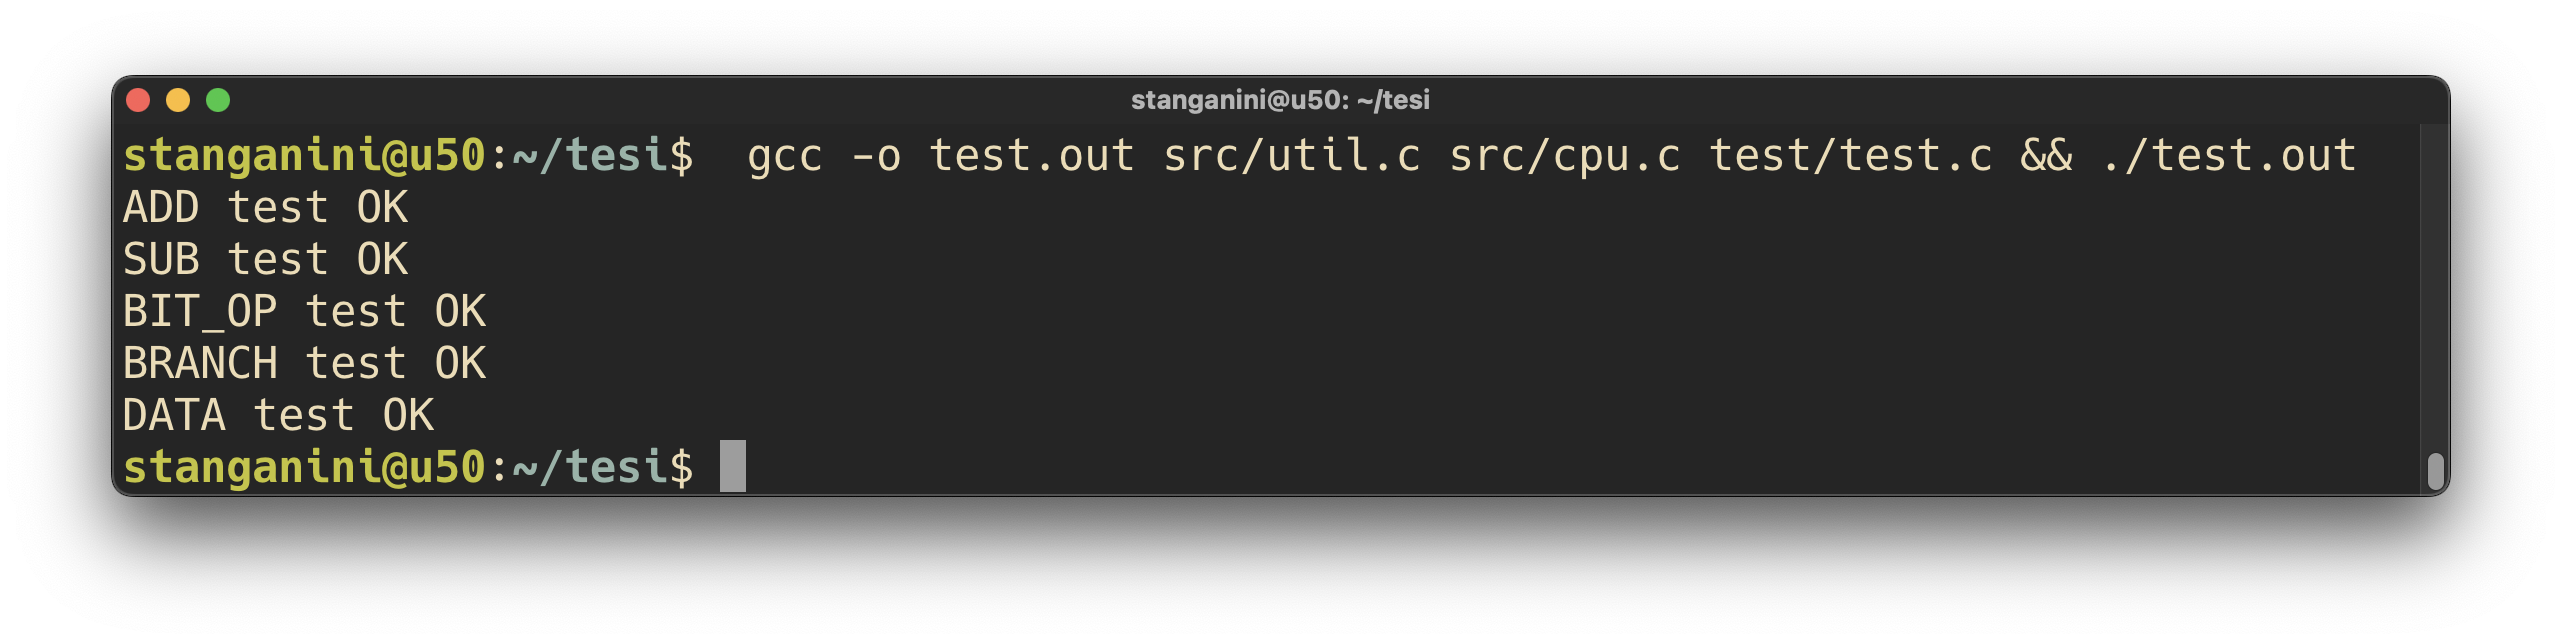
\includegraphics[scale=0.35]{images/Capitolo5/1_im.png}
\caption{Interprete Softcore Risultati}
\label{1curisultati}
\end{figure}

\vspace{0.3cm}

Adesso consideriamo l'esecuzione dell'interprete spiegato nella sez. \ref{Interprete Kernel}, e quindi una singola control unit eseguita all'interno della FPGA.
Per mostrare il risultato è stato cambiato leggermente il codice per passare come argomento al main il nome del file assembler da eseguire.
Possiamo vedere che i risultati ottenuti combaciano con i risultati aspettati:

\begin{lstlisting}[language=C,caption={Risultato Branch}]
#define BRANCH_RESULT 36
\end{lstlisting}

\begin{figure}[h!]
\centering
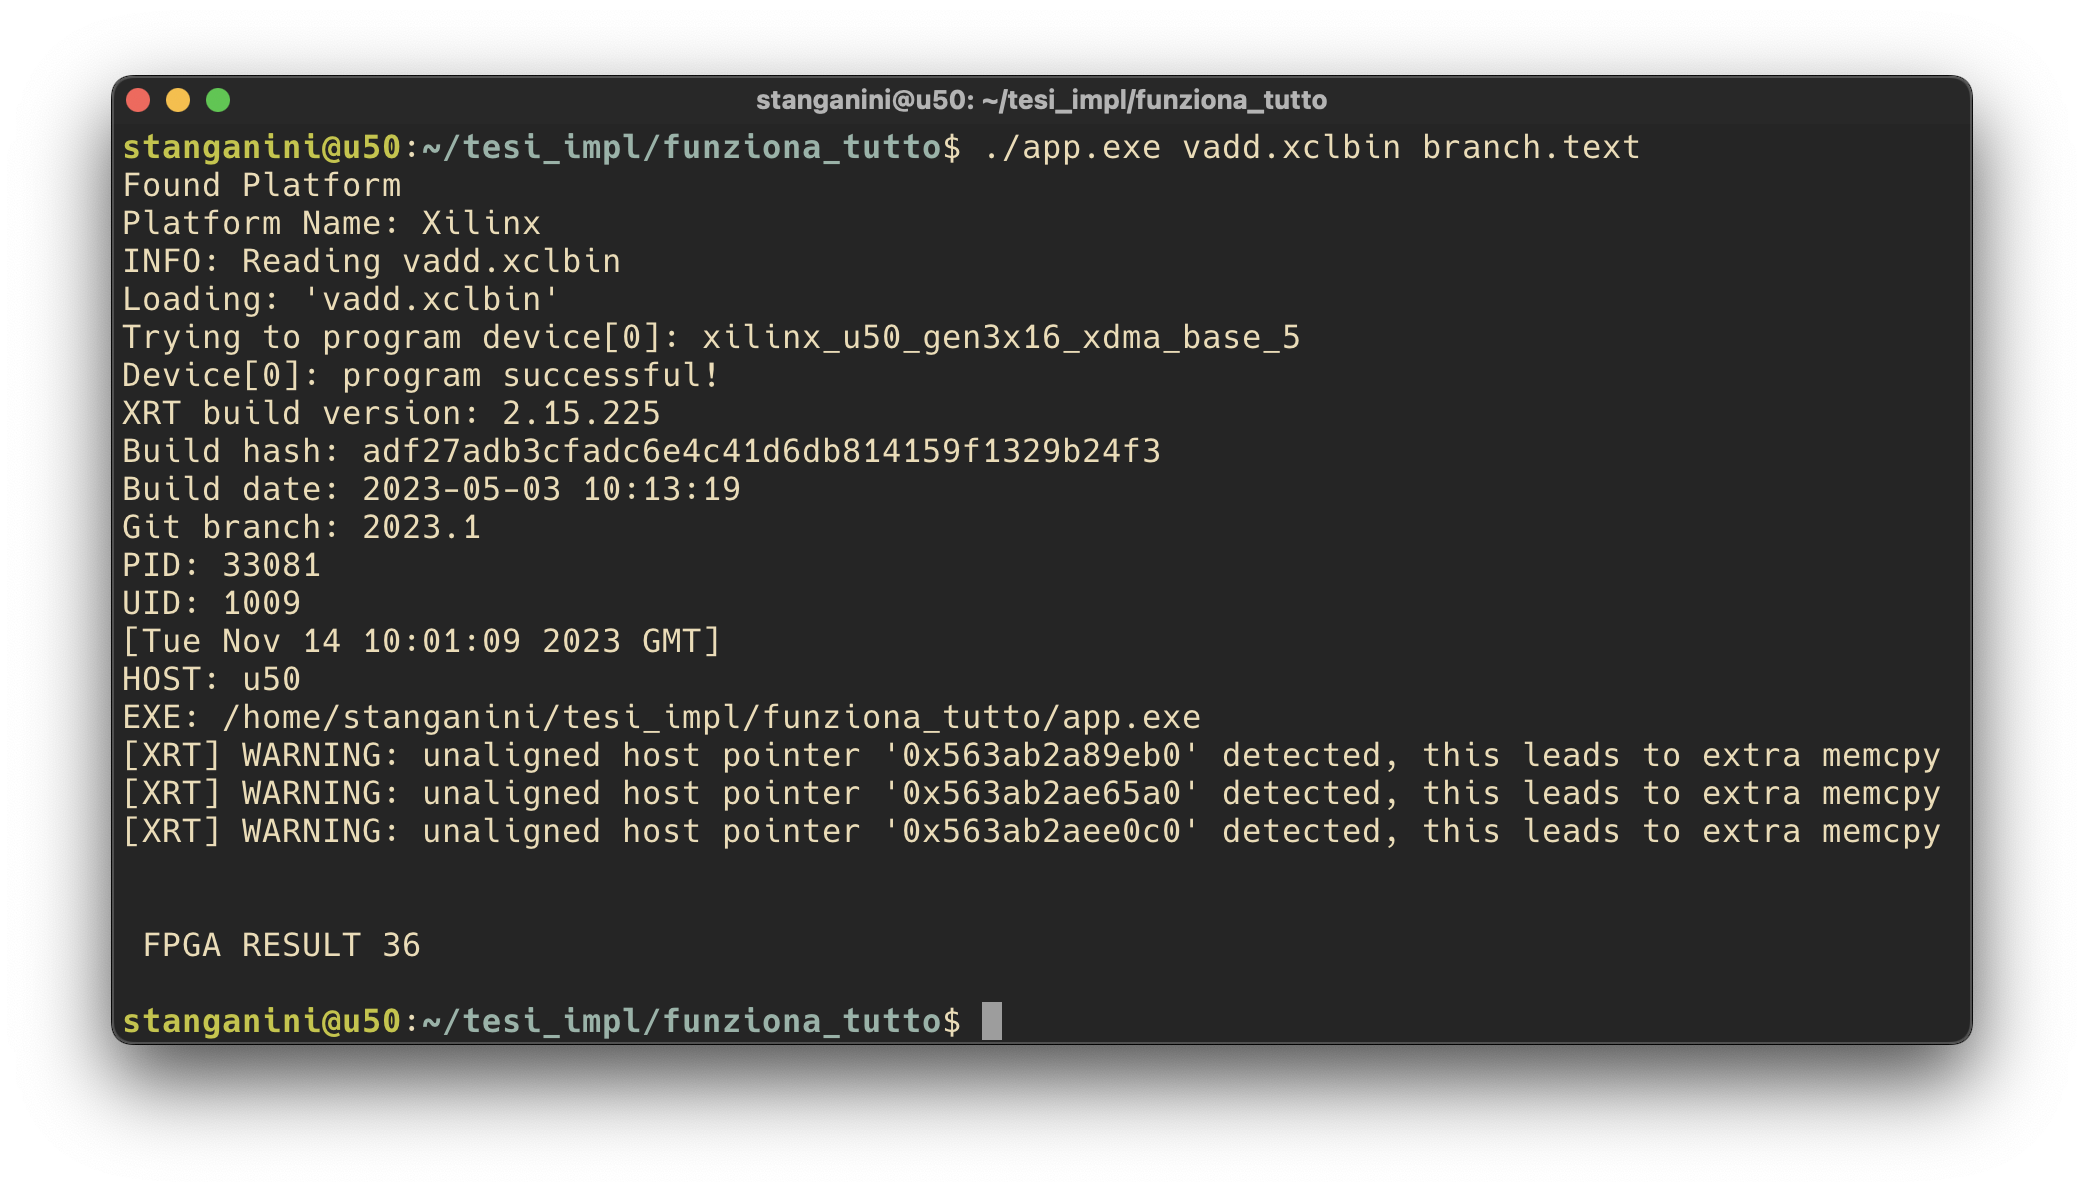
\includegraphics[scale=0.35]{images/Capitolo5/2_im.png}
\caption{Interprete Kernel Risultati}
\label{typeB}
\end{figure}

Questo processo di verifica è stato ripetuto per tutti i file di test, confermando il corretto funzionamento del kernel implementato ed eseguito all'interno della FPGA.

\vspace{0.3cm}


Per la verifica della versione dell'interprete illustrata nella sez.\ref{ControlUnit}, ovvero 4 Control Unit, sono stati usati i file assembler precedentemente spiegati nella fig. \ref{risultatiaspettati}.In particolare, per ciascuna istanza del kernel istanziata, è stato usato un file distinto. 

\vspace{0.3cm}

\noindent Di seguito un immagine dell'esecuzione:

\begin{figure}[h!]
\centering
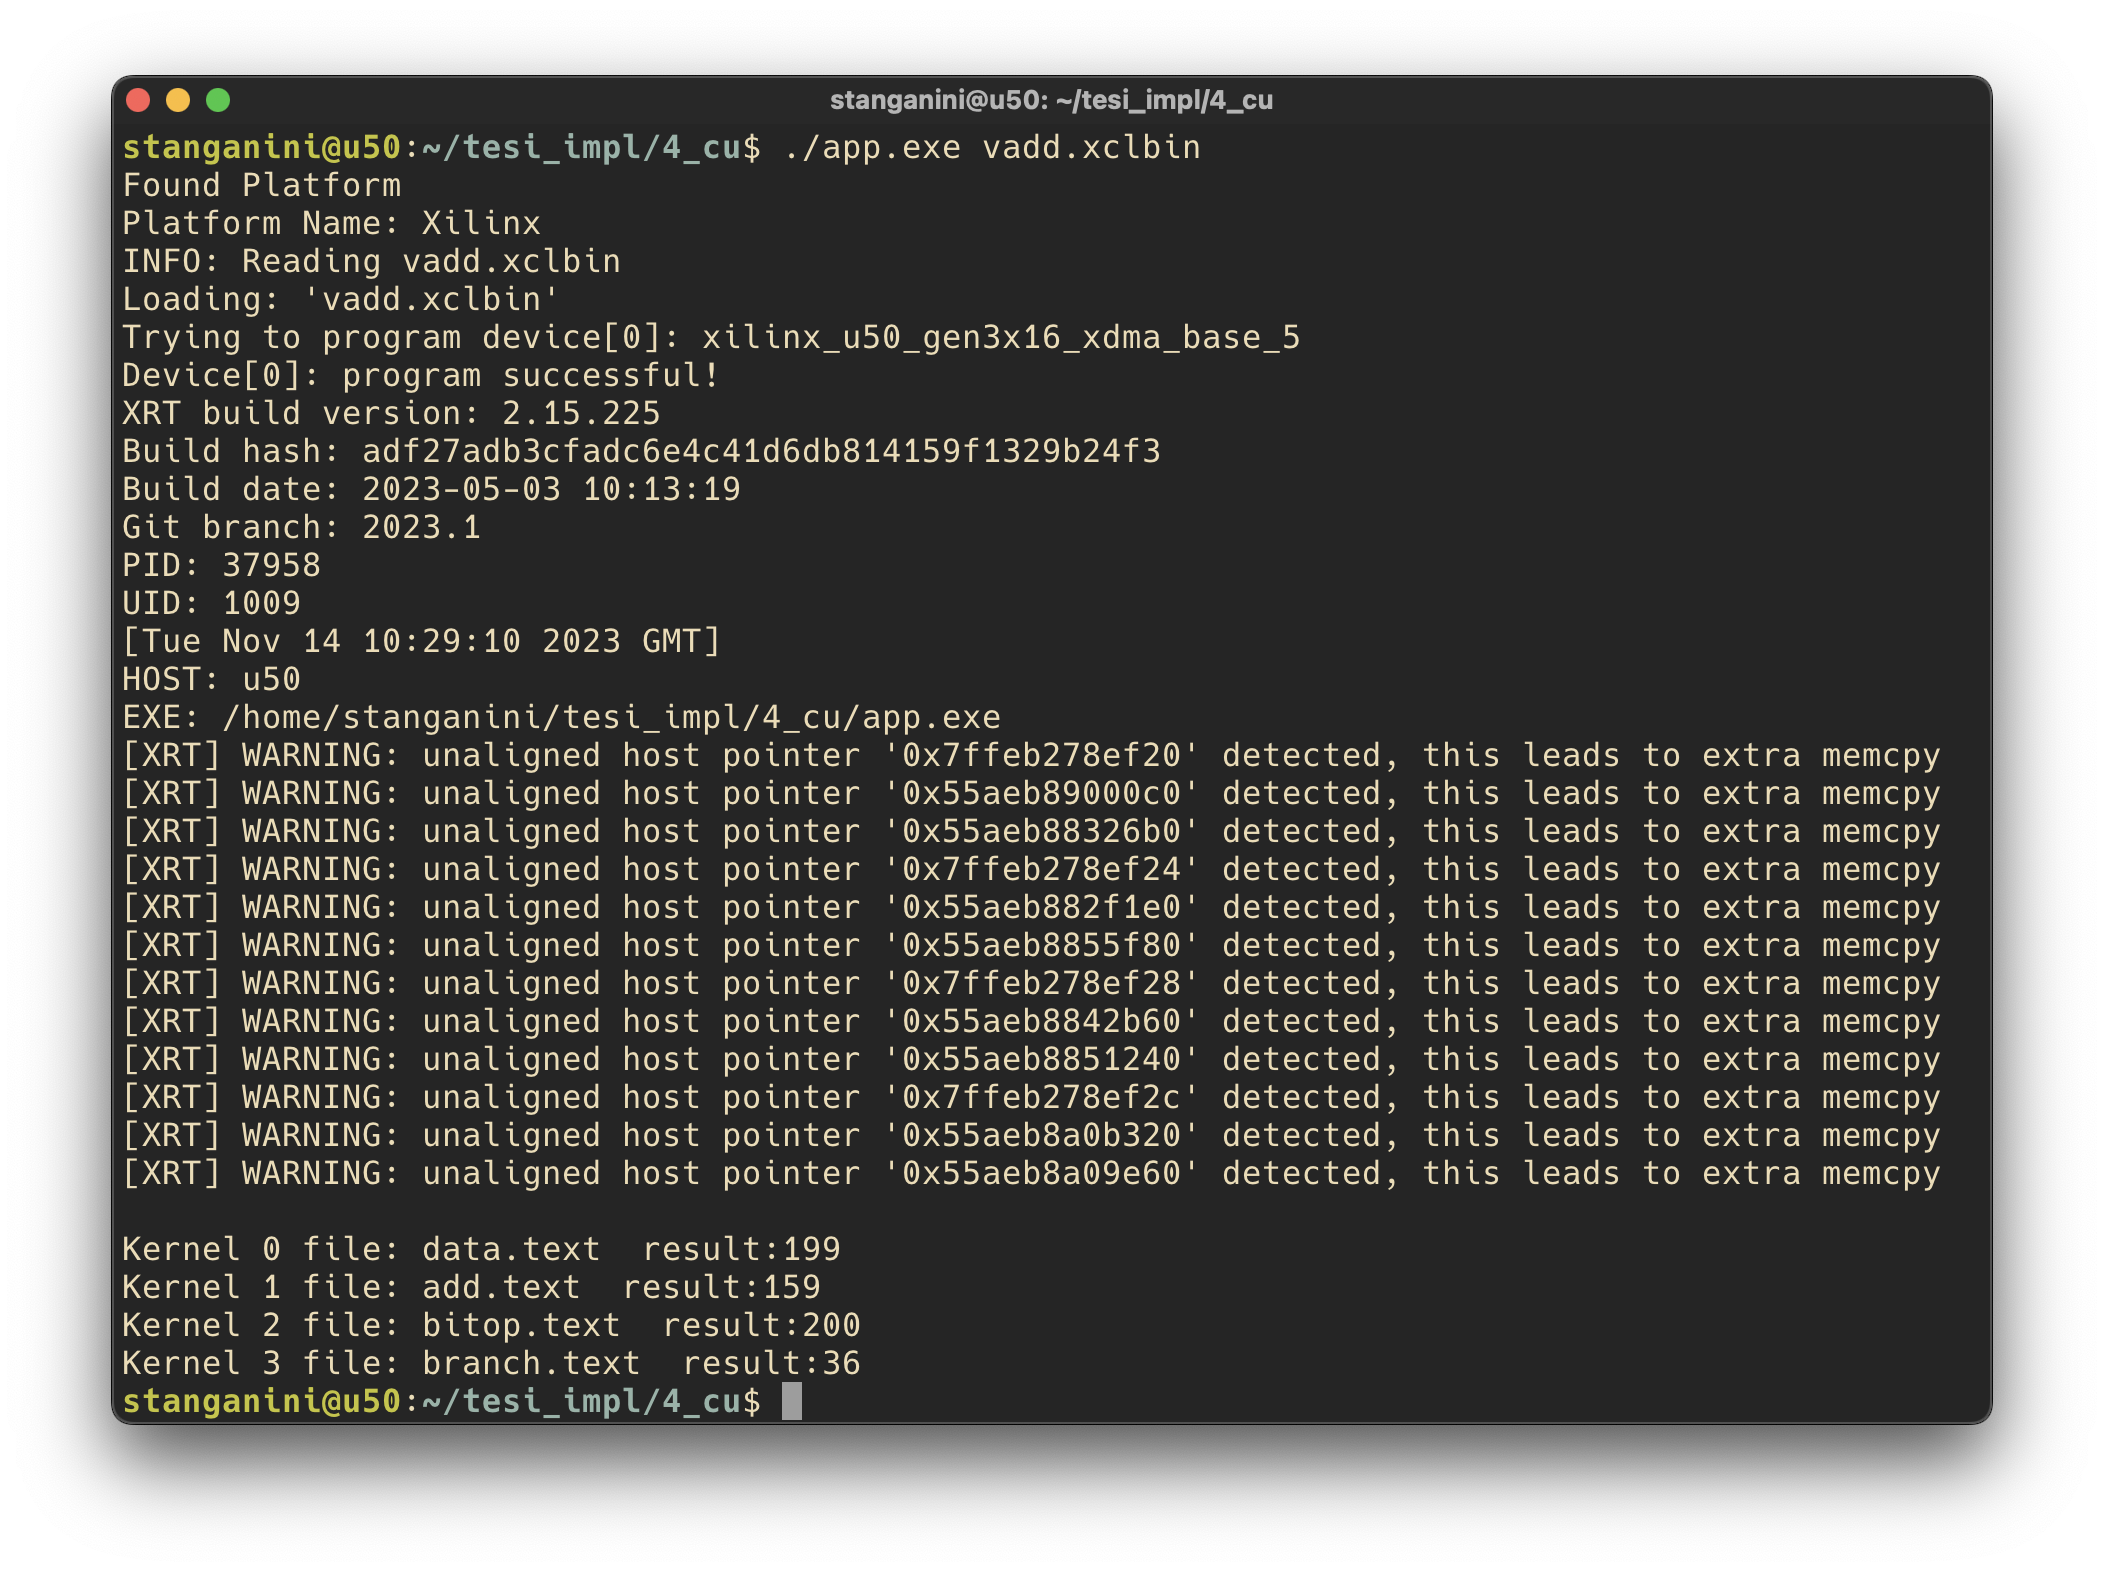
\includegraphics[scale=0.35]{images/Capitolo5/3_im.png}
\caption{Interprete 4 CU Risultati}
\label{4curisultati}
\end{figure}

\noindent Possiamo constatare che i risultati ottenuti combaciano con i risultati attesi, confermando la corretta esecuzione delle 4 istanze dell'interprete all'interno della FPGA che eseguono ciascuna un suo programma diverso dagli altri.

\vspace{0.3cm}

\noindent Per la verifica dell'interprete in virgola mobile illustrato nella sez. \ref{interpretefloating}, considerando che la rappresentazione dei valori in virgola mobile è solo interna all'interprete, per scrivere il file assembly utilizzato nei test, sono stati convertiti i numeri con la virgola usando la funzione di conversione \texttt{f\_to\_i}. Il funzionamento di questa funzione è lo stesso delle funzioni di conversione usate nella sez. \ref{interpretefloating}. Di seguito il programma scritto in C utilizzato per testare il risultato e i valori corretti da usare all'interno delle istruzioni assembler:

\begin{lstlisting}[language=C,label={codicecfloating},caption={Codice valori conversione floating}]
void main()
{
   float a = 177.13;
   printf("a: %d\n", f_to_i(a));

   float b = 231.9999;
   printf("b: %d\n", f_to_i(b));
   
   float c = a + b;

   float d = 99.3;
   printf("d signed: %d\n", f_to_i(d));
   float e = u_to_f(f_to_u(c) | f_to_u(d));

   float f = 20.8;
   printf("f signed: %d\n", f_to_i(f));
   float result = e - f;
   printf("res signed: %d\n", f_to_i(result));
   printf("res: %.6f\n", result);
}
\end{lstlisting}
Di seguito il codice assembler usato per il test dell'interprete in versione floating point: 

\begin{lstlisting}[caption={File Assembler per Test Floating Point},label={assemblerfloating}]
	.text
	.align	2
	.globl	main
	.ent	main
	.type	main, @function       

main:

	addi	r1,r0,1127293256      # r1 = 177.13
	addi	r2,r0,1130889209      # r2 = 231.9999
	add  r1,r1,r2               # r1 = 409.129883
	addi r3,r0,1120311706       # r3 = 99.3
	or r1,r1,r3                 # r1 = 413.200989
	addi r4,r0,1101424230	      # r4 = 20.8
	rsub r1,r4,r1	              # r1 = 392.401001

	.end	main
\end{lstlisting}
Possiamo notare come il file assembler listato in fig. \ref{assemblerfloating} utilizza le stesse operazioni del codice in C listato in fig. \ref{codicecfloating}. Il risultato dell'esecuzione è il valore in virgola mobile \texttt{392.401001}, il quale rappresentato come un \texttt{signed int} è \texttt{1136931668}. Di seguito l'esecuzione dell'interprete in versione Floating Point con il file assembler in listato in fig. \ref{assemblerfloating}:

\clearpage

\begin{figure}[h!]
\centering
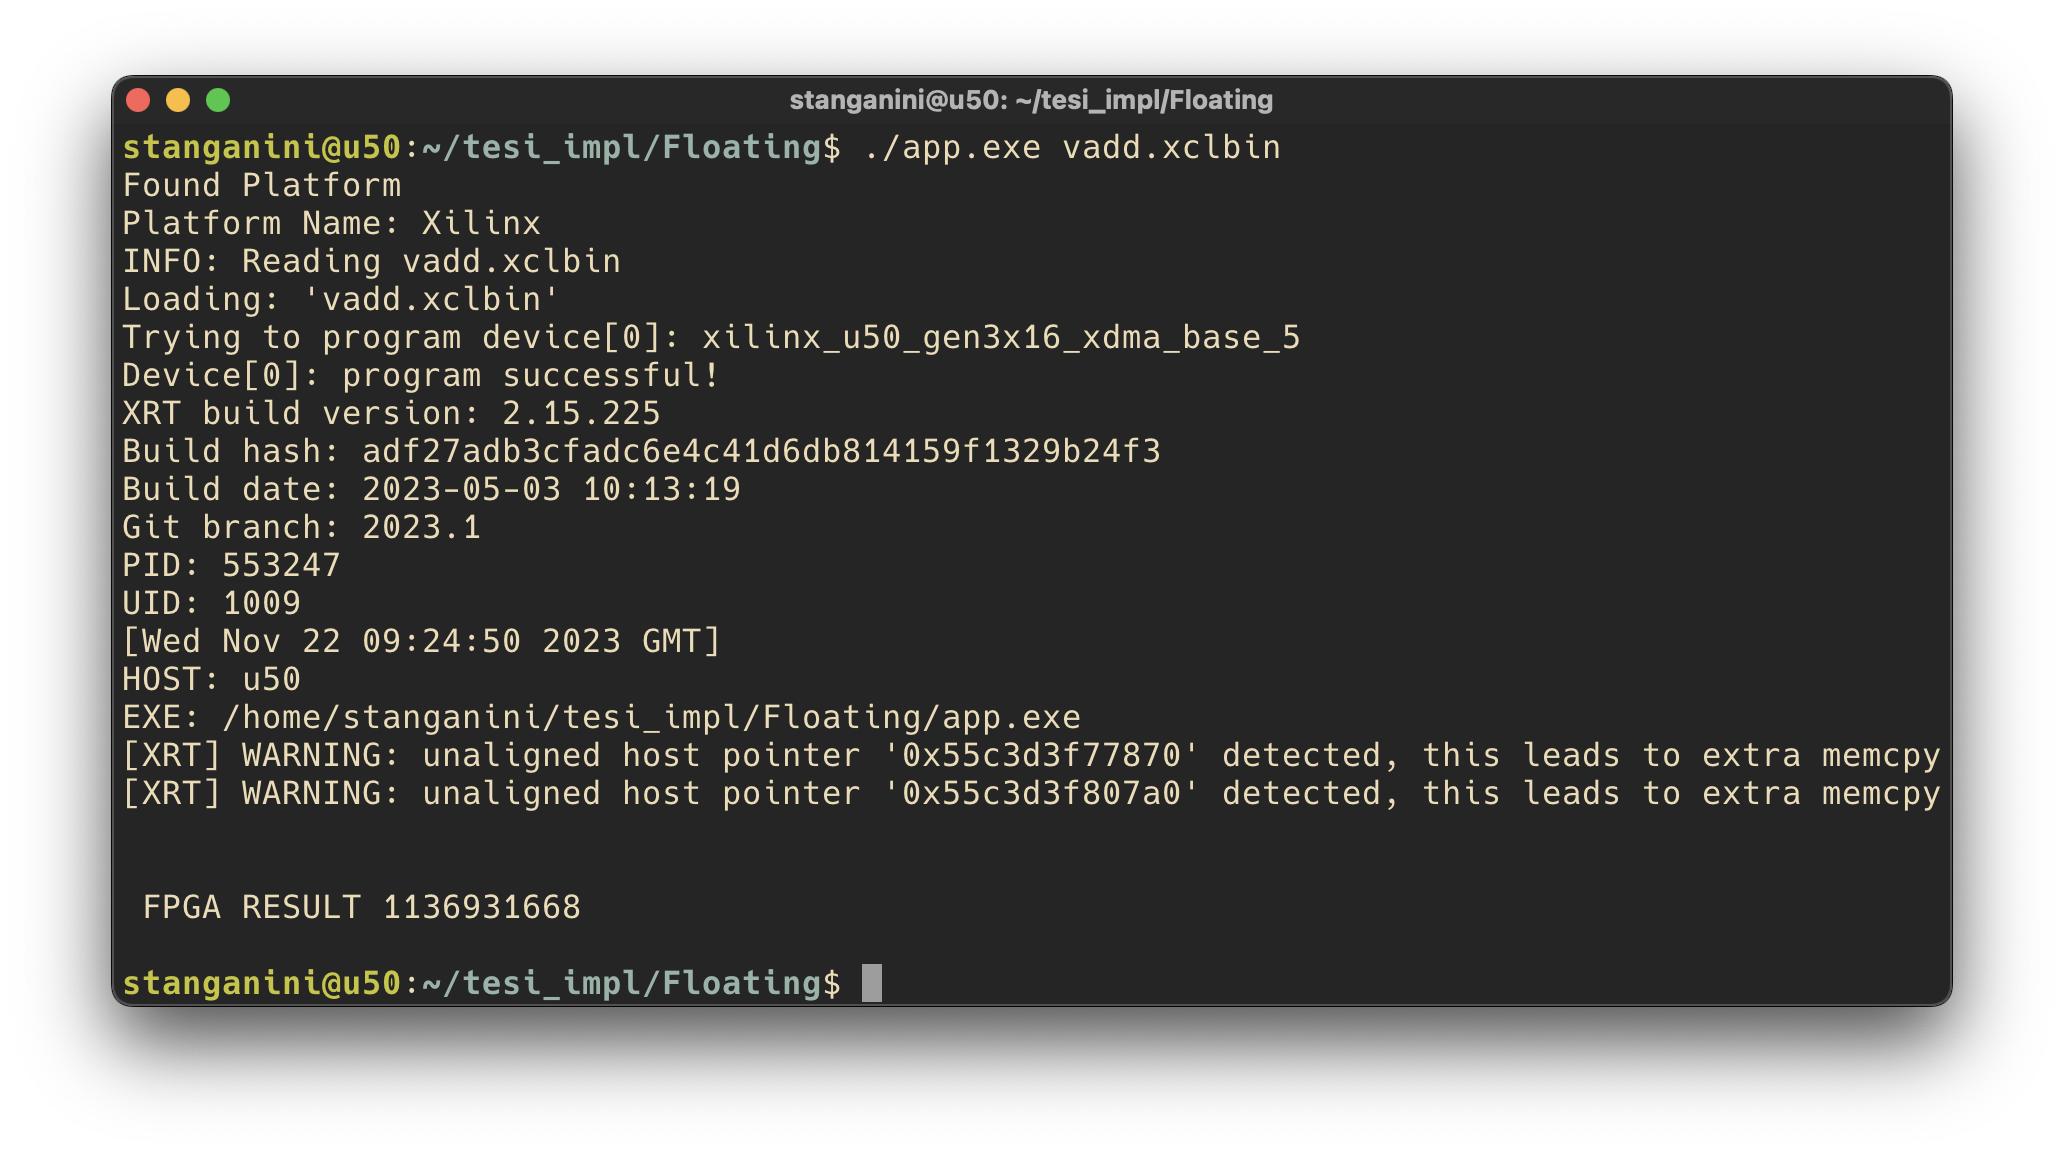
\includegraphics[scale=0.35]{images/Capitolo5/11_im.png}
\caption{Interprete Floating Point Risultati}
\label{4curisultati}
\end{figure}


\vspace{0.3cm}

L'ultima versione dell'interprete da verificare è la quella illustrata della sez. \ref{interpretegpu}. Questo interprete, come precedentemente spiegato, restituisce l'intera memoria dati dopo l'esecuzione. Per questo, al fine di testare il corretto funzionamento di questo interprete, sono stati impiegati i seguenti file per ciascun "core". Di seguito è riportata la lista dei file utilizzati:  

\begin{lstlisting}[language=C]
char const *file[KERNEL_NUMBER] = {
		"gpu_1.text", // v[i] = v[i] + 1,
		"gpu_2.text", // +5
		"gpu_3.text", // -1
		"gpu_4.text", // *2
		"gpu_5.text", // *45
		"gpu_6.text", // & 45
		"gpu_7.text", // | 45
		"gpu_8.text", // >> 1
};
\end{lstlisting}

\vspace{0.3cm}
È evidente come per ciascuna Control Unit sia stato creato un file specifico in linguaggio assembly. Questo file prende un vettore di 15 interi dalla memoria dati, precedentemente inizializzato con numeri casuali. Per ciascun  elemento del vettore viene eseguita un'operazione diversa (come si può notare dai commenti affianco ai nomi dei file). Di seguito il codice assembly usato per compilare ed estrarre il file \texttt{gpu\_2.text}:

\begin{lstlisting}
	.text
	.align	2
	.globl	main
	.ent	main
	.type	main, @function      

main:

	addi	r1,r0,14
	addi	r8,r0,1 
	addi  r2,r0,0
	lwi	 r3,r2,0	
	addi r3,r3,5
	swi  r3,r2,0   
	rsub  r1,r8,r1
	addi  r2,r2,1
	bgei  r1,-20

	.end	main
\end{lstlisting}

Per inizializzare il vettore destinato ai test in memoria che sarà usato dal kernel, si parte dalla posizione \texttt{0} della memoria dati. Per eseguire questa operazione prima di caricare la memoria all'interno dell'interprete è stata apportata una modificata la funzione \texttt{enqueue\_task} spiegata nella fig. \ref{enqueuetask}, inserendo il seguente codice:

\begin{lstlisting}[language=C]
...
for (int i = 0; i < 15; i++)
{
	int32_t n = rand() % 1000;
	data->data[i] = n;
	vector_result[i] = n;
}
...
\end{lstlisting}

È possibile notare che per questioni di semplicità, i numeri si limitano ad un massimo di $1000$. Inoltre è evidente la presenza di un ulteriore vettore,  ovvero \texttt{vector\_result}, il quale viene inizializzato con gli stessi valori della memoria dati. Questo vettore viene calcolato dalla CPU della macchina host con le solite operazioni svolte da ogni istanza dell'interprete dentro la FPGA. Questa procedura ha lo scopo di confrontare il vettore con i risultati ottenuti in memoria per ogni kernel, in modo da verificare il corretto funzionamento. 

\vspace{0.3cm}

\noindent Di seguito è riportato il codice usato nell'interfaccia host per effettuare questa verifica: 

\begin{lstlisting}[language=C++]
...
	struct Memory *data_out[KERNEL_NUMBER];
	int vector_result[KERNEL_NUMBER][15];

	for (int i = 0; i < KERNEL_NUMBER; i++)
	{
		data_out[i] = (struct Memory *)malloc(sizeof(struct Memory));
		enqueue_task(file[i], &q, krnl[i], context, data_out[i], vector_result[i]);
	}

	OCL_CHECK(err, err = q.finish());

	std::cout << "\n";

	for (int i = 0; i < KERNEL_NUMBER; i++)
	{
		make_result(vector_result[i],i);
		compare(data_out[i],vector_result[i], i);
		free(data_out[i]);
	}

	return EXIT_SUCCESS;
}
\end{lstlisting}

Per ciascun kernel è presente un vettore risultati, i quali come spiegato precedentemente vengono inizializzati all'interno della funzione \texttt{enqueue\_task}. Successivamente attraverso la funzione \texttt{make\_result()}, vengono calcolati i valori lato host per ogni kernel seguendo le operazioni specificate nei file. In fine, per verificare che i risultati ottenuti siano in linea con i risultati attesi all'interno di \texttt{vector\_result}, viene utilizzata la funzione \texttt{compare}. Di seguito è riportata l'implementazione di tale funzione:

\begin{lstlisting}[language=C++]
void compare(struct Memory *data, int32_t *vector_result, int n)
{
	bool cmp = true;

	for (int i = 0; i<15; i++) 
		if (data->data[i] != vector_result[i])
			cmp = false;

	if (cmp) 
		std::cout << " Kernel: " << n << " Test Passed\n";
	else 
		std::cout << " Kernel: " << n << " Test Failed\n";
}
\end{lstlisting}
Possiamo notare come la funzione accetti come input la memoria restituita dall'interprete e il vettore dei risultati, calcolato sulla macchina host. Successivamente effettua un confronto tra i due e stampa il risultato del risultato ottenuto.

\vspace{0.3cm}

\noindent Di seguito è riportata l'immagine con il risultato dell'esecuzione del codice precedentemente descritto: 

\begin{figure}[h!]
\centering

\includegraphics[scale=0.45]{images/Capitolo5/4_im.png}
\caption{Interprete GPU Risultati}
\label{gpurisultati}
\end{figure}

\clearpage 

\section{Utilizzo FPGA}
\label{utilizzofpga}
Durante il processo di compilazione, il compilatore \texttt{v++} genera il file \texttt{.xclbin.link} \texttt{\_summary}. Questo  file contiene le informazioni sull'utilizzo effettivo delle risorse del chip della FPGA. Nel seguito di questa sezione verranno presentati i risultati ottenuti dalle diverse versioni dell'interprete. È importante notare che tutti i dati ottenuti durante questa fase siano stati letti utilizzando il software offerto da Vitis ovvero \texttt{vitis\_analyzer}. 

\vspace{0.3cm}

\noindent Di seguito i risultati relativi alla versione dell'interprete spiegata nella sez. \ref{Interprete Kernel}, corrispondente ad una singola istanza dell'interprete all'interno della FPGA:

\begin{figure}[h!]
\centering
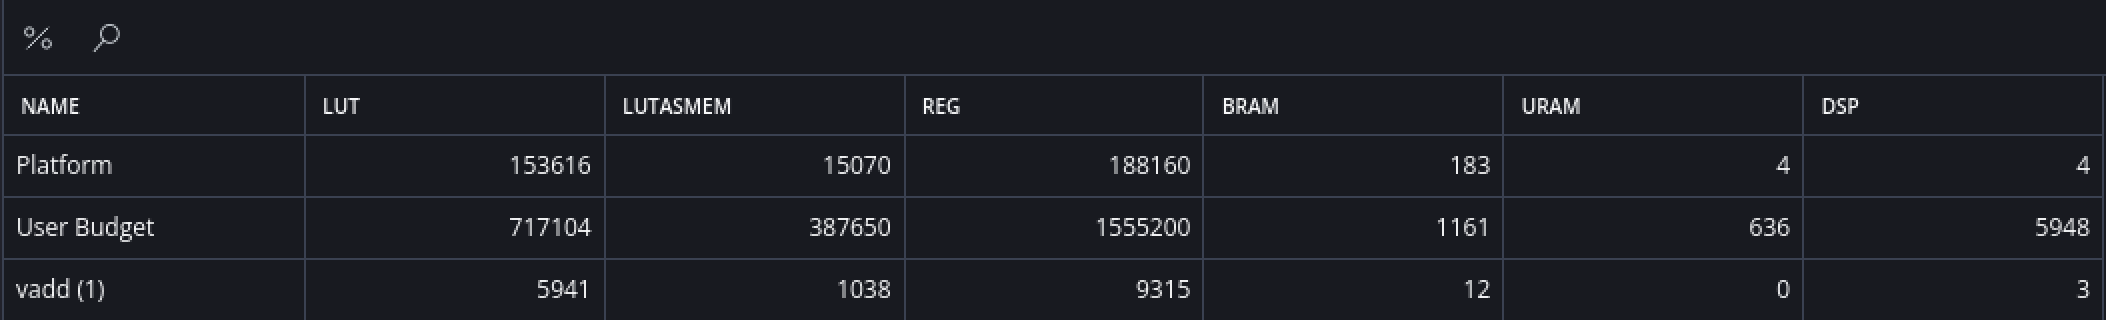
\includegraphics[scale=0.40]{images/Capitolo5/5_im.png}
\caption{Utilizzo FPGA 1 Control Unit}
\label{utlizzo1cu}
\end{figure}

\vspace{0.3cm}

\noindent Nella tabella è possibile vedere i seguenti campi:

\begin{itemize}
    \item \textbf{LUT} (Look-Up Table): Gli elementi fondamentali per una FPGA per realizzare circuiti logici. Le LUT sono delle tabelle di ricerca usate per implementare funzioni logiche. Presentano un numero di ingressi fisso e generano un'uscita in base ai valori memorizzati, che variano a seconda della funzione che si vuole realizzare \cite{sitoLUT}.
    \item \textbf{LUTASMEM}: Sono una versione delle LUT che può funzionare come memoria lettura/scrittura.
    \item \textbf{REG} (Register): Nel contesto delle FPGA, i registri sono gruppi di flip-flop utilizzati per memorizzare i dati temporanei. Possono essere utilizzati per sincronizzare segnali, memorizzare risultati intermedi e altro ancora \cite{sitoREG}. 
    \item \textbf{BRAM} (Block RAM): Blocchi di memoria RAM configurabili all'interno della FPGA. Queste memorie sono utilizzate per memorizzare i dati in modo efficiente, migliorando cosi le prestazioni dei circuiti implementati per le FPGA.
    \item \textbf{URAM} (Ultra RAM): Blocchi di memoria RAM ad alte prestazioni progettate per massimizzare larghezza di banda e latenza. Questi tipi di RAM sono disponibili solo su alcune schede FPGA \cite{sitoURAM}.
    \item \textbf{DSP} (Digital Signal Processor): Sono delle ALU solitamente in Floating Point all'interno della FPGA dedicate alle per operazioni matematiche complesse come moltiplicazioni, accumuli e altro ancora \cite{sitoDSP}. 
\end{itemize}

\noindent È possibile notare come le righe della tabella in fig. \ref{utlizzo1cu}, riguardano la disponibilità totale delle risorse della piattaforma, quanto l'utente ha a disposizione in termini delle risorse totali e quanto il kernel compilato occupa di queste risorse.
È importante sottolineare che la quantità delle risorse disponibile dipende direttamente dal tipo di scheda utilizzata, nel nostro caso la Alveo U50 \ref{Specifiche-U50}.

\vspace{0.3cm}

\noindent Di seguito sono riportati i risultati dell'occupazione della FPGA per la versione dell'interprete spiegata nella sez. \ref{ControlUnit}, ovvero 4 istanze del kernel compilate all'interno della FPGA:

\begin{figure}[h!]
\centering
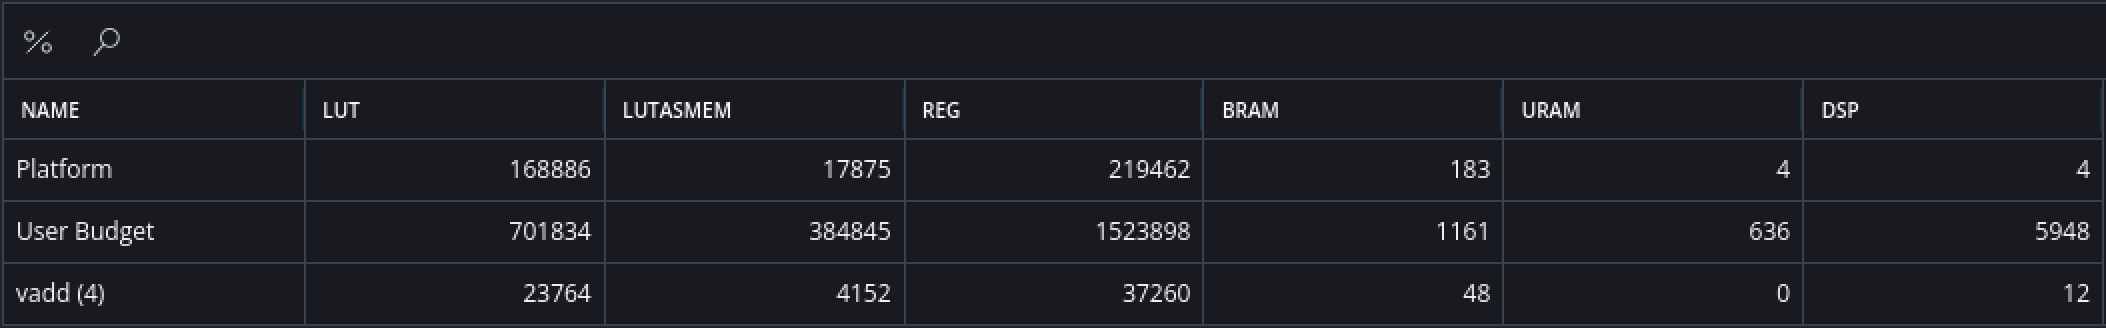
\includegraphics[scale=0.40]{images/Capitolo5/6_im.png}
\caption{Utilizzo FPGA 4 Control Unit}
\label{utilizzo4cu}
\end{figure}
 
Mettendo a confronto le tabelle in fig. \ref{utlizzo1cu} e in fig. \ref{utilizzo4cu} possiamo concludere che:

\begin{itemize}
    \item LUT: L'utilizzo è di circa $0.8 \%$ nella versione a 1 istanza del kernel, rispetto a circa $3.4 \%$ nella versione a 4.
    \item LUTASMEM: L'utilizzo è del $0.3 \%$ contro un $1 \%$ nella versione a 4 istanze del kernel.
    \item REG: L'utilizzo è del $0.6 \%$ dei registri rispetto a $2.5 \%$ per la versione a 4 kernel.
    \item BRAM: L' utilizzo è del $1 \%$ contro un $4 \%$ 
    \item URAM: L'utilizzo è del $0 \%$ in tutti e due casi.
    \item DSP: L'utilizzo è del $0.05 \%$ contro $0.2 \%$.
\end{itemize}
Va notato che le percentuali menzionate sono state approssimate per migliorare la leggibilità.
Da questi risultati emerge che, l'occupazione delle risorse cresce con l'istanziazione di più kernel all'interno della FPGA. Inoltre si osserva che le risorse utilizzate non aumentano esattamente in modo lineare con il numero di kernel, ma che una parte di risorse è impiegata anche per gestire la complessità introdotta dall'aumentare delle componenti hardware all'interno del chip della FPGA.

\vspace{0.3cm}

\clearpage

\noindent Di seguito sono riportati i risultati di occupazione della versione dell'interprete descritta in sez. \ref{interpretegpu}: 

\begin{figure}[h!]
\centering
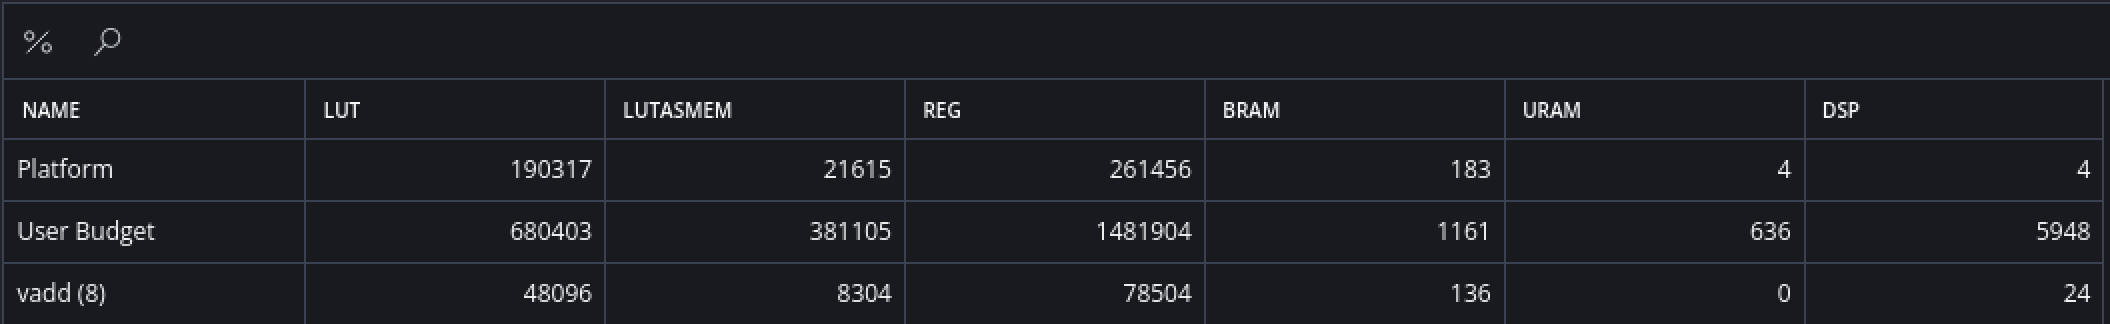
\includegraphics[scale=0.40]{images/Capitolo5/7_im.png}
\caption{Utilizzo FPGA 8 Control Unit}
\label{utilizzo4cu}
\end{figure}

In questo caso notiamo un utilizzo del $7 \%$ delle LUT, $5 \%$ dei registri, e $12 \%$ di utilizzo delle BRAM. Questi risultati sono coerenti con il trend di crescita dell'utilizzo delle risorse osservato fin'ora. Inoltre va notato come con la scheda usata permetta di compilare ancora maggiore di kernel rispetto al massimo di 8 raggiunti nel codice citato in precedenza. Con  l'utilizzo delle risorse osservato finora, è possibile stimare che circa 56 kernel possono essere inseriti nell'FPGA utilizzata per gli esperimenti (la scheda Alveo U50 \ref{Alveo}).

\vspace{0.3cm}

\noindent Di seguito sono riportati i risultati dell'occupazione della FPGA per la versione dell'interprete spiegata nella sez. \ref{interpretefloating}, ovvero l'interprete con la rappresentazione interna dei valori in virgola mobile:

\begin{figure}[h!]
\centering
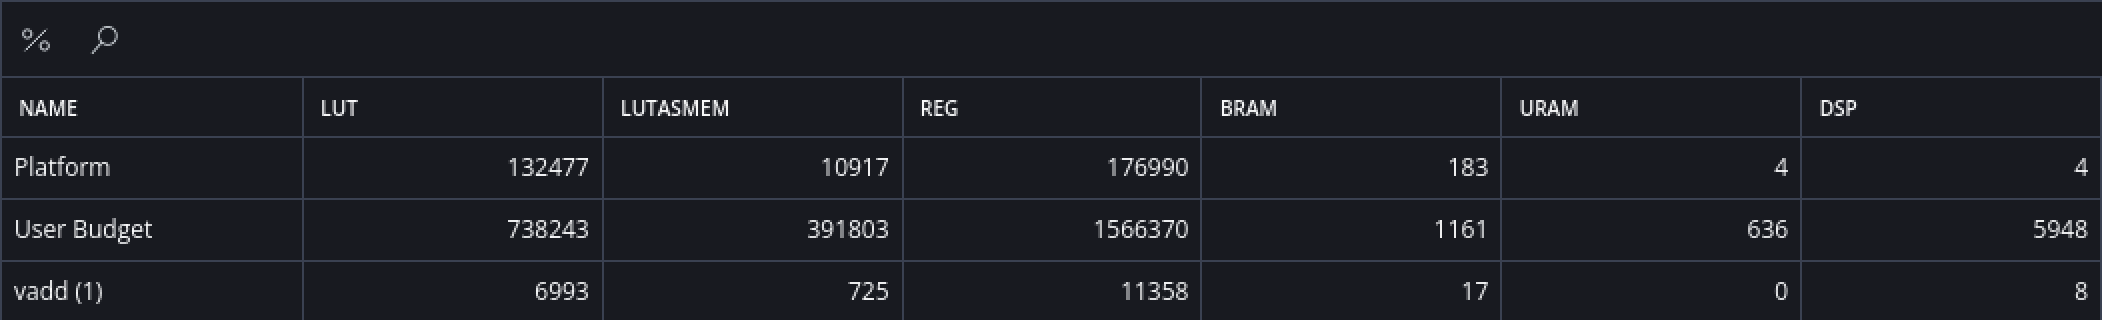
\includegraphics[scale=0.40]{images/Capitolo5/12_im.png}
\caption{Utilizzo FPGA Floating Point}
\label{utilizzo4cu}
\end{figure}

Possiamo notare, come, rispetto all'utilizzo della versione ad 1 CU senza virgola mobile, listata in fig. \ref{utlizzo1cu}, è presente un maggior utilizzo dei DSP, questo perché come spiegato precedentemente nella definizione delle DSP, queste ALU vengono usate per il calcolo in virgola mobile. Di conseguenza, come prevedibile, si è registrato un aumento del loro utilizzo rispetto alla versione senza virgola mobile.

\vspace{0.3cm}

È importante sottolineare che, durante lo sviluppo di questo interprete , l'ottimizzazione nell'occupazione delle risorse della FPGA non era un obbiettivo fondamentale. Nella documentazione del processore Microblaze \cite{sitoMicroblaze}, vengono mostrate delle statistiche sull'utilizzo delle risorse nelle varie schede FPGA del mercato con varie implementazioni del processore, sviluppate direttamente dagli sviluppatori del processore utilizzando un linguaggio RTL. Viene mostrato che il processore occupa mediamente circa 3000 LUT. Pertanto, possiamo concludere che anche se il nostro interprete implementi solo un sotto insieme di tutte le istruzioni assembler, e sia scritto in un linguaggio di alto livello e convertito in hardware tramite HLS offerto da Vitis, con un utilizzo  medio di 5600 LUT, possiamo considerarci soddisfatti, tenendo anche conto della facilità di configurazione e estensione che questa soluzione offre.

\vspace{0.3cm}

Durante lo sviluppo del progetto, è stata prestata abbastanza attenzione all'utilizzo delle BRAM all'interno della FPGA. Questo è stato fatto al fine di minimizzare l'uso della memoria globale DDR, la quale trovandosi fuori dal chip FPGA, aggiunge latenza e e richiede circuiti hardware aggiuntivi per gestire il processo di comunicazione.
Per verificare l'effettivo posizionamento dentro la BRAM delle strutture dati utilizzate all'interno del interprete, sono state sviluppate due versioni. In entrambe è presente un sottoinsieme ancora più piccolo di istruzioni per questioni di semplicità, ma in una versione per la computazione si utilizzavano direttamente i parametri passati dall'OpenCl e caricati nella memoria DDR. Nell'altra versione, si è seguito il paradigma illustrato nella sez. \ref{Interprete Kernel} e listato nella fig. \ref{funzioneinterprete} dove i parametri sono copiati su strutture dati dichiarate all'interno della funzione.

Di seguito il codice della versione che non effettua la copia locale dei parametri:

\begin{lstlisting}[language=C]
void interprete(struct Memory *mem, struct Registers *reg, uint32_t *out, ap_uint<32> my_size)
{
pragma HLS INTERFACE m_axi port = mem bundle = gmem
pragma HLS INTERFACE m_axi port = reg bundle = gmem
pragma HLS INTERFACE m_axi port = out bundle = gmem
pragma HLS INTERFACE ap_ctrl_hs port = return

	while (reg->pc < my_size)
		run_instruction(mem->instr[reg->pc], 
						mem, 
						reg, 
						mem->instr, 
						false);

	out[1] = reg->r[1];
}
\end{lstlisting}

In questa implementazione, si noti l'uso diretto dei parametri istanziati dalla parte host e caricati nella DDR.

\vspace{0.3cm}

Di seguito i risultati di occupazione delle due versioni:

\begin{figure}[h!]
\centering
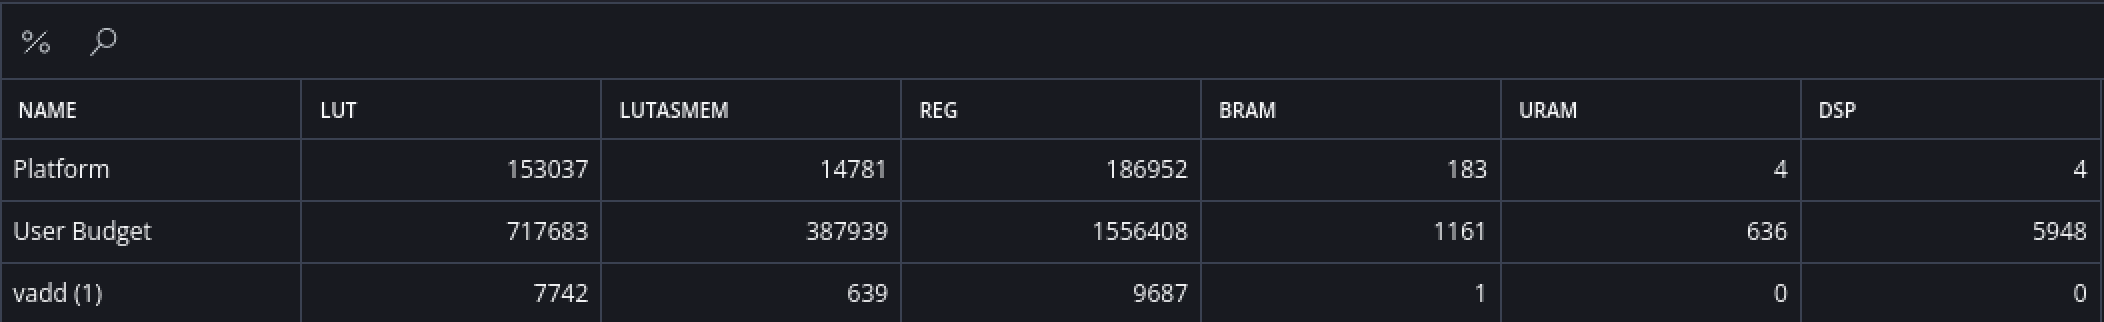
\includegraphics[scale=0.40]{images/Capitolo5/9_im.png}
\caption{Utilizzo senza copia locale dei parametri}
\label{nopragma}
\end{figure}

\begin{figure}[h!]
\centering
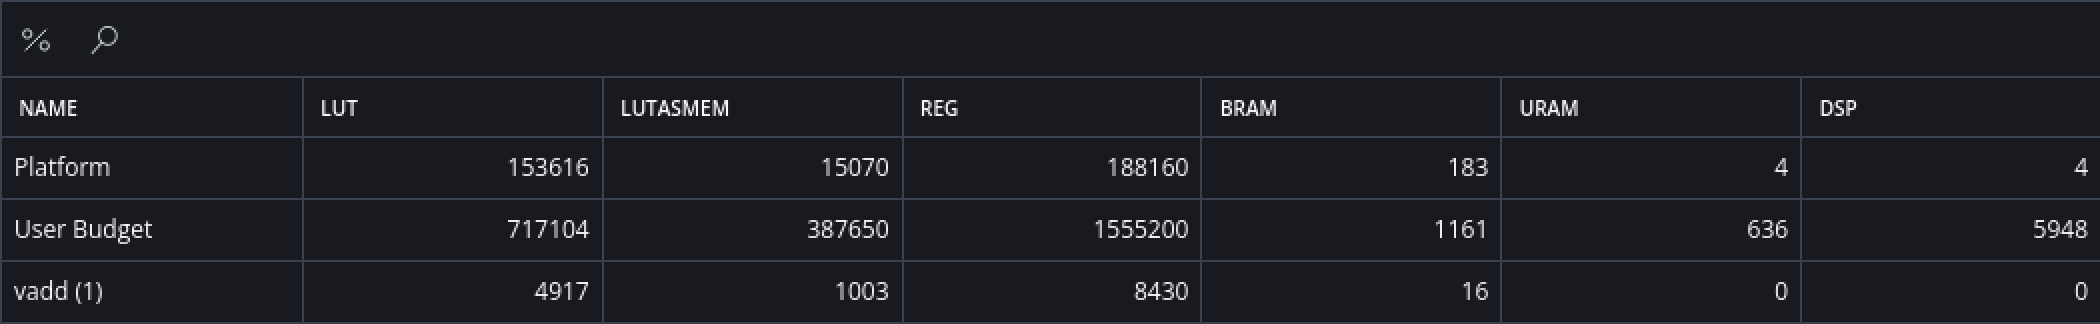
\includegraphics[scale=0.40]{images/Capitolo5/8_im.png}
\caption{Utilizzo con copia locale dei parametri}
\label{pragma}
\end{figure}

È possibile notare come l'utilizzo delle BRAM sale da 1 a 16 con l'implementazione che prevede la copia locale dei parametri. Questo conferma  che le strutture utilizzate per effettuare la copia dei parametri sono istanziate all'interno del chip della FPGA, consentendo un esecuzione più efficiente e veloce del kernel.

\vspace{0.3cm}

\clearpage

\section{Execution Summary}
Attraverso l'utilizzo del file \texttt{xrt.ini}, come indicato dalla documentazione \cite{sitoDocumentazioneVitis}, è possibile abilitare la generazione del file \texttt{xrt.run\_summary}. All'interno di questo file sono raccolte le informazioni sugli eventi registrati durante l'esecuzione della FPGA.

\vspace{0.3cm}

\noindent Di seguito l'immagine del \texttt{run\_summary}, aperto tramite lo strumento \texttt{vitis\_analyzer}, delle informazione riguardanti dell'esecuzione del codice spiegato nella sez. \ref{Interprete Kernel} (1 istanza):

\begin{figure}[h!]
\centering
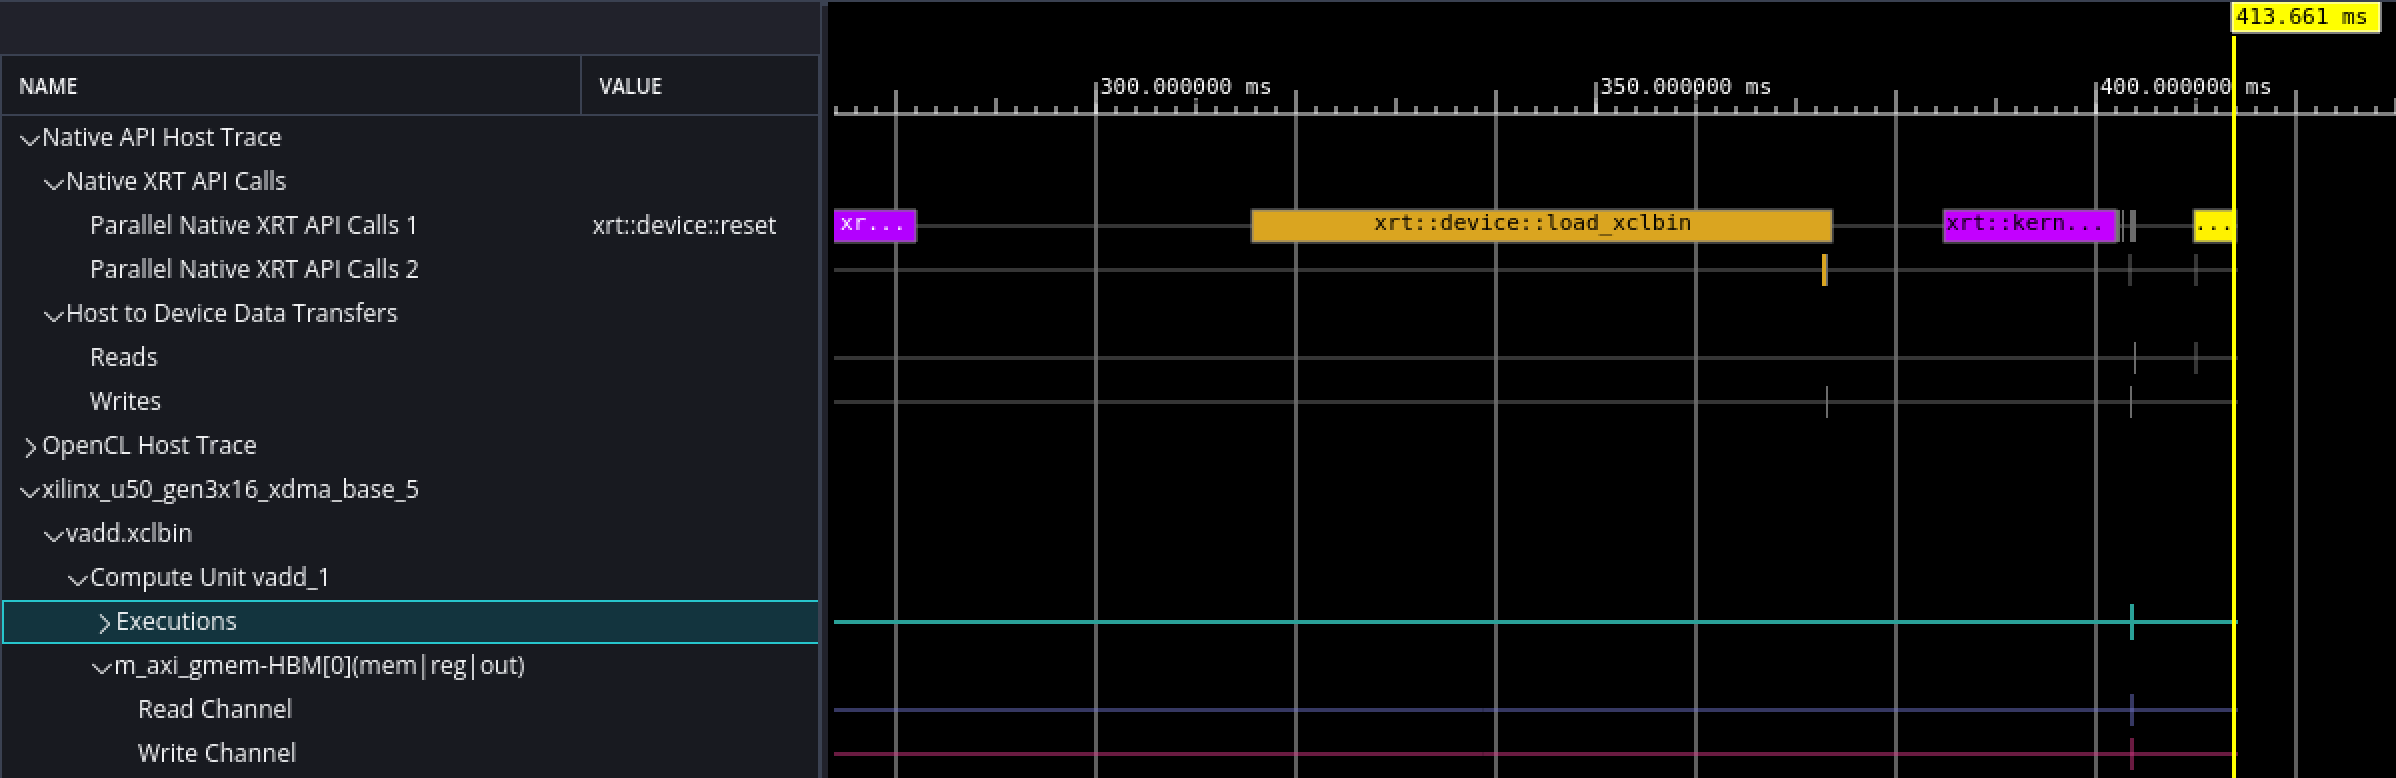
\includegraphics[scale=0.35]{images/Capitolo5/10_im.png}
\caption{run\_summary 1 Kernel}
\label{1curunsummary}
\end{figure}

\noindent All'Interno di questo grafico, possiamo notare come l'esecuzione del programma lato host, che comprende il caricamento del file \texttt{.xclbin}, l'inserimento e l'estrazione dei dati dalla memoria globale, e l'esecuzione effettiva del kernel, dura $413$ ms.
È interessante notare come gran parte del tempo di esecuzione è dedicato alle chiamate API dal lato host (in fig.  \ref{1curunsummary} nella parte superiore), mentre il tempo effettivo dove inizia l'esecuzione della Control Unit (in fig.  \ref{1curunsummary})  evidenziata con nome \texttt{Executions}), avviene in un intervallo molto breve. Ciò è dovuto al fatto che il programma assembly utilizzato per l'esecuzione che possiamo osservare nel grafico in fig. \ref{1curunsummary}, è composto di poche istruzioni e, di fatto, non contiene cicli di queste istruzioni. 

\vspace{0.3cm}

In un ottica futura, nel contesto di una possibile "soft GPU" che sfrutti questi softcore, il caricamento del kernel (contenuto nel file \texttt{.xclbin}) verrebbe eseguito una sola volta per tutti i core, per poi poter caricare volta per volta lo stato della memoria, dei registri, con i relativi programmi da eseguire. Questo permetterebbe di togliere l'overhead associato al dover programmare nuovamente l'FPGA ogni volta che si desidera eseguire un programma.
